\newpage

\section{Metodología}

\subsection{Materiales a utilizar}
\begin{enumerate}
    \item Kit Fischertechnik
    \item Cable de red
    \item Resistencias variadas
    \item Pulsadores
    \item Matriz de leds
    \item Plotter 
    \item Jumpers
\end{enumerate}


\subsection{Punzonadora}
\subsubsection{Configuración de temporizador variable}
Se configura al timer 1 con un overflow de 1s, pero un contador de overflow regresivo configurable, permitiendo realizar una acción después de una cantidad especificada overflows consecutivos del temporizador. 

\subsubsection{Manejo de estados}
Utilizando este temporizador variable, se realiza la lógica de cambio de estado utilizando una máquina de estados y diferentes condicionales para ajustar por los distintos tipos de carga. 

\begin{figure}[H]
  \centering
  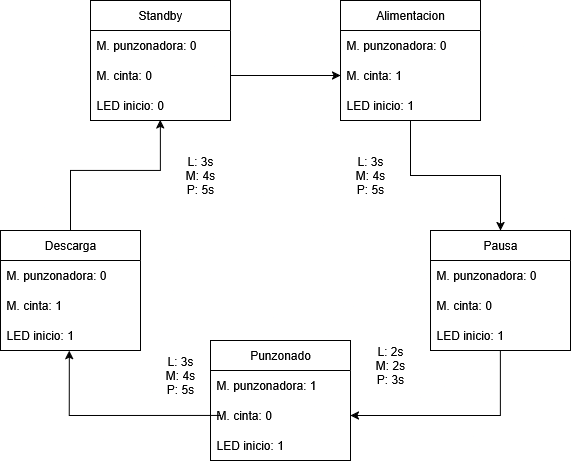
\includegraphics[width=\linewidth]{./Anexos/Metodologia/Punzonadora/Diagrama de estados.png}
  \caption{Diagrama de estados para punzonadora. Fuente: Elaboración propia.}
  \label{fig:punzoadora_estados}
\end{figure}

\subsubsection{Botones, LEDs,  y debouncing}
Con la máquina de estados funcionando, se realiza un circuito indicador y de comando para poder iniciar el proceso, y configurar el tipo de carga que se va a manejar. Se implementa el timer 2 para realizar un deboucing de los pulsadores. 

\subsubsection{USART}
Implementado las funcionalidades de USART del anexo \ref{anexo:USART_Asincrono_con_Ring_Buffer}, se configura USART para mostrar un mensaje de inicio, y además indicar al usuario el estado actual de la máquina.

\subsection{Matriz}

\subsubsection{Objetivo inicial}
El objetivo es controlar una \textbf{matriz de LEDs 8×8 (1088AS)}. Se comienza con lo básico: encender un solo LED indicando su fila y su columna. A partir de ahí se progresa hasta dibujar cuadros completos y finalmente animaciones.

\subsubsection{Encendiendo un solo LED}
Para ubicar cada LED se prepararon \textbf{lookup tables} en memoria de programa. Una tabla indica el \textbf{puerto} asociado a cada fila y columna y otra el \textbf{pin} dentro de ese puerto. El flujo es simple: se cargan en registros la fila y la columna deseadas, se usa el \textbf{puntero Z} para leer puerto y pin desde las tablas y se construye una \textbf{máscara de bits}. Primero se lee el valor actual del puerto y luego se aplica la máscara para encender o apagar el bit. Cuando fila y columna comparten puerto se agrega un cuidado extra para no alterar otros bits. Recordatorio importante: las \textbf{filas} se activan con \texttt{0} y las \textbf{columnas} con \texttt{1}, por lo que se emplean máscaras invertidas según corresponda.

\subsubsection{Multiplexado y dibujo de cuadros}
Resuelto el encendido individual, se pasa al \textbf{multiplexado} para refrescar la matriz de forma continua y dar la ilusión de múltiples LEDs encendidos. Al principio se usó un retardo activo y luego se contempló el uso de un temporizador e interrupciones. Los \textbf{frames} se guardan como mapas de bits 8×8 donde 0 es apagado y 1 encendido. Una subrutina recorre las 64 posiciones, compara el bit del cuadro (con desplazamientos como \texttt{LSR}), decide si encender el LED combinando la máscara con los puertos y aplica operaciones lógicas para modificar solo los LEDs necesarios.

\subsubsection{De cuadros a animación}
Con la rutina de dibujo funcionando, basta con llamarla en bucle para mantener la imagen. Así se pueden mostrar figuras estáticas como una cara sonriente. Para animaciones, por ejemplo texto desplazándose, el \textbf{Timer 2} se configura con un desborde cada 100\,ms. Entre desbordes la rutina de dibujo corre a alta velocidad (del orden de microsegundos). En cada desborde se incrementa un \textbf{puntero índice} que desplaza el origen de lectura de los datos del cuadro y produce el efecto de movimiento sobre la matriz. Además se agrega una condición de comparación que retorna la animación al inicio cuando se llega al final. Véase anexo \ref{anexo:Configuracion_Timer_1}


\subsubsection{Base para el control por estados}
Con estas piezas el sistema ya enciende LEDs individuales, dibuja cuadros desde memoria y ejecuta animaciones cuadro a cuadro. Este es el \textbf{motor de visualización básico} que luego se conecta a la \textbf{máquina de estados} y a la \textbf{entrada por USART} para seleccionar entre texto desplazante, imágenes estáticas u otros patrones. Véase anexo \ref{anexo:Maquina_de_Estados} y anexo \ref{anexo:USART_Asincrono_con_Ring_Buffer}

\newpage

\subsection{Conversor}
En este ejercicio se buscó visualizar en el osciloscopio la \textbf{señal 7}, correspondiente a una onda triangular (verificada a través de python en el anexo \ref{anexo:Senal_para_conversor_digital_analogo}).

Para ello se empleó un conversor digital-analógico (DAC) basado en una red de resistencias R-2R, con un total de 17 resistencias de valores intercambiados entre 10k $\Omega$ y 20k $\Omega$. El puerto D del microcontrolador Arduino (pines digitales 0 a 7) se conectó directamente a las entradas del DAC, permitiendo convertir los valores digitales en niveles de tensión analógicos.

En la programación del Arduino se implementó una \textit{Look-Up Table} (LUT), en la cual se almacenaron los valores correspondientes a la forma de onda triangular. Posteriormente, estos datos se recorrieron utilizando el puntero \textbf{Z}, generando así la secuencia digital que, al pasar por el DAC, produjo la señal triangular observada en el osciloscopio.

\subsection{Plotter}

\subsubsection{Mapeo de comandos}
Para el plotter se tomaron las instrucciones de la tabla mostrada en el anexo \ref{anexo:Comandos_Plotter} y se mapean las máscaras correspondientes a cada instrucción a variables internas para mejorar legibilidad de código.

\subsubsection{Interprete de secuencias}
Utilizando las variables definidas previamente, se realizan series de instrucciones predefinidas para desplazamientos y figuras, guardando dichas secuencias en FLASH. Produciendo algo que podría ser descrito como un lenguaje de programación interno dentro del mismo programa, donde al plotter se le indicia el tipo de acción, y por cuando tiempo realizarla. 

\subsubsection{Creación secuencia para círculo por Python}
Para evitar realizar operaciones trigonométricas complejas con el microcontrolador debido a las limitaciones claras limitaciones del lenguaje, se implementa un programa en Python para utilizar operaciones trigonométricas e imprimir el ``programa'' equivalente en assembler para el plotter para obtener resultados con mejor resolución. Ver anexo \ref{anexo:Plotter_Python}

\subsubsection{USART}
Una vez implementado el interprete de comandos, se configura la comunicación USART para mostrar un menú de opciones, y comandar al plotter a través de este para realizar diferentes trazados.


